\chapter{Análisis de requisitos}

Referenciando directamente al PMBOK \cite{pmbok} se define la recopilación de requisitos como:

\begin{quote}
	\textit{
	“[...]el proceso que consiste en definir y documentar las necesidades de los interesados
	a fin de cumplir con los objetivos del proyecto. El éxito del proyecto depende directamente
	del cuidado que se tenga en obtener y gestionar los requisitos del proyecto y del
	producto”
	}
\end{quote}

Como bien se indica en la cita anterior, el éxito de un proyecto está estrechamente relacionado con la calidad y precisión empleados en el proceso de recogida, análisis y gestión de los requisitos del mismo. Esto hace que imperiosa la necesidad de llevar a cabo los procesos mencionados con extrema minuciosidad y cuidado.

\bigskip

A Continuación se estudiarán las necesidades del proyecto en términos de funcionalidades y objetivos deseables para así obtener una idea sobre el alcance del mismo. Para ello se realizará la identificación y descripción de los múltiples requisitos que se deberán cumplir, separándolos según su índole y relacionándolos con los casos de uso apropiados.

\section{Identificación de los requisitos del sistema}

El primer paso a la hora de realizar correctamente el proceso de análisis de requisitos es dedicar el tiempo necesario para comprender cuales son los objetivos y alcance reales del mismo. Para ello se han llevado a cabo varias reuniones con los tutores previas a la reunión del proyecto en las que se ha discutido cual sería el producto final buscado así como los requisitos que dicho producto tendría que cumplir para estar a la altura de dicho ideal. En sucesivas reuniones iterativas con ambos tutores se ha logrado tener una idea común del alcance a cumplir mediante el refinamiento de los requisitos, buscando la mínima ambigüedad posible en su definición.

\subsection{Actores}

El primer paso que se debe afrontar dentro del proceso de análisis de requisitos es la identificación de los actores que intervendrán en la ejecución del sistema de una forma u otra. Un actor representa cualquier tipo de rol interpretado por una persona, dispositivo o sistema externo que tendrá capacidad de interactuar con nuestro producto. En este caso particular, la definición de los actores es sencilla y directa: el único rol que se debe definir es el del \textbf{usuario que interacciona con el videojuego} descrito en esta memoria. En aras de hacer una especificación formar realizaremos la descripción de los actores en la siguiente tabla:



\begin{center}
	\begin{tabular}{ | p{3cm} | p{10cm} | } 
		\hline
		\textbf{ID} & Actor-01 \\
		\hline 
		\textbf{Nombre} & Jugador \\ 
		\hline
		\textbf{Descripción} & 
		Este actor representa al usuario que interaccionará con el videojuego, realizando partidas contra otro jugador o el agente implementado así como ejecutando el proceso de simulación de partidas que el agente usará como proceso de aprendizaje.\\
		\hline 
	\end{tabular}
\end{center}

\subsection{Casos de uso}


Una vez especificados los actores que interactúan con el sistema el siguiente paso es identificar y especificar los diferentes casos de uso. Dichos casos de uso nos permitirán centrarnos luego en los requisitos del sistema partiendo de una base sólida.


\bigskip

Se definirá caso de uso como \cite{modelado_referencia} una secuencia de acciones, incluyendo variantes, que ejecuta un sistema para producir un resultado observable de valor para un actor. De esta forma se pueden utilizar los casos de uso para definir el comportamiento deseado durante la etapa de desarrollo realizando una abstracción que permitirá que los miembros involucrados en el proyecto puedan hacer referencia a ellos sin preocuparse de detalles de bajo nivel. De esta forma se facilitarán discusiones sobre el funcionamiento deseado del proyecto, incluido el análisis de requisitos.

\bigskip

De este mismo modo, lo que se hará a continuación es reconocer las diferentes acciones que pueden llevar a cabo los actores, en este caso solamente uno, sobre el sistema. Haciendo una primera aproximación a esta definición de un modo informal podemos considerar las siguientes acciones: Un usuario deberá ser capaz de seleccionar entre las diferentes acciones a realizar dentro del entorno del juego, lo que dará lugar a la ejecución de otros casos de uso diferentes (\textbf{seleccionar la opción a ejecutar dentro del videojuego}). Las diferentes opciones darán lugar a casos de uso diferentes ya que el usuario podrá competir con otro usuario con el mismo rol (\textbf{ competición de jugador humano contra jugador humano}) o competir con el agente entrenado (\textbf{ competición de jugador humano contra agente}). Finalmente se podrá hacer que el agente compita con otra versión de sí mismo (\textbf{competición de agente contra agente}). Además esta ultima acción se puede llevar a cabo sin que el actor visualice el proceso exponiendo solo los resultados con el fin de llevar a cabo el proceso de aprendizaje del agente.

\bigskip

\begin{figure}
	\centerline{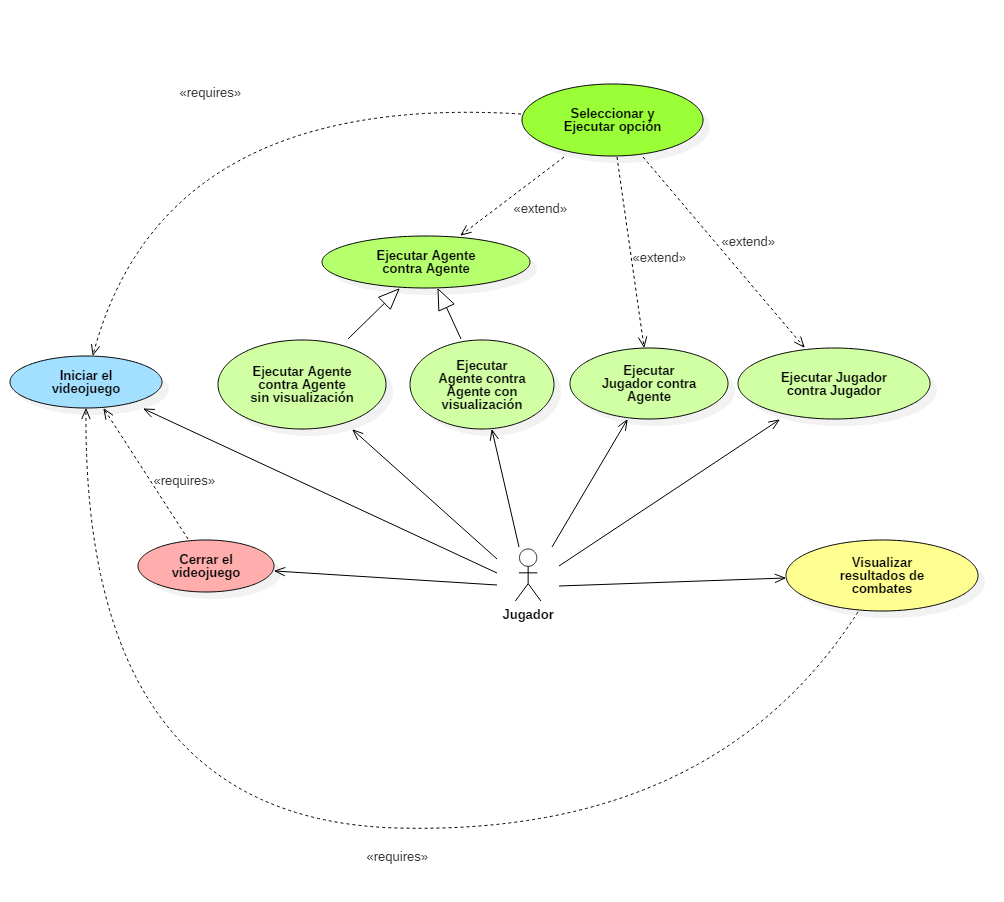
\includegraphics[width=20cm]{diagramas/casosDeUsoCropped.png}}
	\caption{Diagrama de casos de uso}
	\label{casos_de_uso}
\end{figure}

\clearpage

En la figura \ref{casos_de_uso} se muestra el diagrama de casos de uso a partir del cual podremos realizar una definición formal de los mismos. En dicha figura se han agrupado por colores los casos de uso con características similares para facilitar su comprensión y visualización. En este caso se utilizan el color azul y rojo para abrir y cerrar el programa, colores verdes para los diferentes tipos de ejecuciones posibles del combate y el amarillo para ver los resultados de los combates realizados en una ejecución.

\bigskip

A continuación se muestran los casos de uso especificados de manera formal. La notación utilizada para la identificación de los diferentes casos de uso será \textbf{CU\footnote{en referencia a Caso de Uso}-\textit{N\footnote{en referencia al Número asociado al mismo}}}. Los campos presentes en cada descripción contarán con un identificador, nombre, descripción y una prioridad. El nivel de prioridad podrá tener uno de los siguientes tres valores con su significado asociado:

\begin{itemize}
\item \textbf{Vital}: Es fundamental para completar el proyecto.
\item \textbf{Importante}: Aumenta de forma significativa la calidad y funcionamiento del proyecto pero no tiene la cualidad de indispensable.
\item \textbf{Deseable}: Extiende el proyecto pero no debería ser una prioridad.
\end{itemize}

\bigskip



\newcounter{contador_casos_de_uso}
\setcounter{contador_casos_de_uso}{1}

\begin{center}
	\begin{tabular}{ | p{3cm} | p{10cm} | } 
		\hline
		
			\textbf{ID} & CU-\arabic{contador_casos_de_uso}
			\refstepcounter{contador_casos_de_uso} \\
		
		\hline 
		
			\textbf{Nombre} &
			Iniciar el videojuego \\ 
		
		\hline
		
			\textbf{Descripción} & 
			El usuario ejecuta el programa.\\
		
		\hline 
		
			\textbf{Prioridad} &
			Vital\\ 
		
		\hline
	\end{tabular}
\end{center}

\begin{center}
	\begin{tabular}{ | p{3cm} | p{10cm} | } 
		\hline
		
		\textbf{ID} & CU-\arabic{contador_casos_de_uso}
		\refstepcounter{contador_casos_de_uso} \\
		
		\hline 
		
		\textbf{Nombre} &
		Cerrar el videojuego \\ 
		
		\hline
		
		\textbf{Descripción} & 
		El usuario cierra el programa.\\
		
		\hline 
		
		\textbf{Prioridad} &
		Vital\\ 
		
		\hline
	\end{tabular}
\end{center}

\begin{center}
	\begin{tabular}{ | p{3cm} | p{10cm} | } 
		\hline
		
		\textbf{ID} & CU-\arabic{contador_casos_de_uso}
		\refstepcounter{contador_casos_de_uso} \\
		
		\hline 
		
		\textbf{Nombre} &
		Seleccionar y Ejecutar opción \\ 
		
		\hline
		
		\textbf{Descripción} & 
		El usuario escoge una de las opciones posibles para ser ejecutada.\\
		
		\hline 
		
		\textbf{Prioridad} &
		Vital\\ 
		
		\hline
	\end{tabular}
\end{center}


\begin{center}
	\begin{tabular}{ | p{3cm} | p{10cm} | } 
		\hline
		
		\textbf{ID} & CU-\arabic{contador_casos_de_uso}
		\refstepcounter{contador_casos_de_uso} \\
		
		\hline 
		
		\textbf{Nombre} &
		Ejecutar Agente contra Agente \\ 
		
		\hline
		
		\textbf{Descripción} & 
		El usuario escoge una de las opciones en las que el agente compite contra otra versión de sí mismo.\\
		
		\hline 
		
		\textbf{Prioridad} &
		Vital\\ 
		
		\hline
	\end{tabular}
\end{center}


\begin{center}
	\begin{tabular}{ | p{3cm} | p{10cm} | } 
		\hline
		
		\textbf{ID} & CU-\arabic{contador_casos_de_uso}
		\refstepcounter{contador_casos_de_uso} \\
		
		\hline 
		
		\textbf{Nombre} &
		Ejecutar Agente contra Agente con visualización \\ 
		
		\hline
		
		\textbf{Descripción} & 
		El usuario escoge la opción de visualizar un combate entre un agente y otra versión de sí mismo.\\
		
		\hline 
		
		\textbf{Prioridad} &
		Vital\\ 
		
		\hline
	\end{tabular}
\end{center}

\begin{center}
	\begin{tabular}{ | p{3cm} | p{10cm} | } 
		\hline
		
		\textbf{ID} & CU-\arabic{contador_casos_de_uso}
		\refstepcounter{contador_casos_de_uso} \\
		
		\hline 
		
		\textbf{Nombre} &
		Ejecutar Agente contra Agente sin visualización \\ 
		
		\hline
		
		\textbf{Descripción} & 
		El usuario escoge la opción de simular un combate entre un agente y otra versión de sí mismo sin realizar una visualización del mismo.\\
		
		\hline 
		
		\textbf{Prioridad} &
		Vital\\ 
		
		\hline
	\end{tabular}
\end{center}

\begin{center}
	\begin{tabular}{ | p{3cm} | p{10cm} | } 
		\hline
		
		\textbf{ID} & CU-\arabic{contador_casos_de_uso}
		\refstepcounter{contador_casos_de_uso} \\
		
		\hline 
		
		\textbf{Nombre} &
		Ejecutar Jugador contra Agente\\ 
		
		\hline
		
		\textbf{Descripción} & 
		El usuario escoge la opción que le permite competir contra el agente.\\
		
		\hline 
		
		\textbf{Prioridad} &
		Vital\\ 
		
		\hline
	\end{tabular}
\end{center}


\begin{center}
	\begin{tabular}{ | p{3cm} | p{10cm} | } 
		\hline
		
		\textbf{ID} & CU-\arabic{contador_casos_de_uso}
		\refstepcounter{contador_casos_de_uso} \\
		
		\hline 
		
		\textbf{Nombre} &
		Ejecutar Jugador contra Jugador\\ 
		
		\hline
		
		\textbf{Descripción} & 
		El usuario escoge la opción que le permite competir contra otro usuario.\\
		
		\hline 
		
		\textbf{Prioridad} &
		Importante\\ 
		
		\hline
	\end{tabular}
\end{center}

\begin{center}
	\begin{tabular}{ | p{3cm} | p{10cm} | } 
		\hline
		
		\textbf{ID} & CU-\arabic{contador_casos_de_uso}
		\refstepcounter{contador_casos_de_uso} \\
		
		\hline 
		
		\textbf{Nombre} &
		Visualizar resultados de combates\\ 
		
		\hline
		
		\textbf{Descripción} & 
		El usuario visualiza los resultados acumulados de los combates que han ocurrido en la ejecución del programa.\\
		
		\hline 
		
		\textbf{Prioridad} &
		Deseable\\
		
		\hline
	\end{tabular}
\end{center}


\subsection{Especificación de requisitos}

Una vez definidos los casos de uso se puede proceder a realizar un análisis detenido de cada uno de ellos para así extraer los requisitos que se deben cumplir para hacer posible su ejecución. Esta sección estará dedicada a clasificar y describir con el menor grado de ambigüedad posibles cada uno de los requisitos del proyecto. Para este fin utilizaremos el estándar IEEE830 \cite{ieee}, en el que se define la diferenciación entre tres tipos de requisitos:

\begin{itemize}
\item \textbf{Requisitos de información}: Identificados con códigos de la forma RI-\textit{N}
\item \textbf{Requisitos funcionales}: Identificados con códigos de la forma RF-\textit{N}
\item \textbf{Requisitos no funcionales}: Identificados con códigos de la forma RNF-\textit{N}
\end{itemize}

Algunos de los campos que se utilizarán para describir los requisitos son comunes, tales como el identificador (ID), nombre, descripción y criticidad. En aras de mantener un buen nivel de consistencia se utilizará una escala similar a la de la importancia de los casos de uso para definir la criticidad, pudiendo tomar la misma los siguientes valores:

\begin{itemize}
	\item \textbf{Vital}: Es fundamental para completar el proyecto.
	\item \textbf{Importante}: Aumenta de forma significativa la calidad y funcionamiento del proyecto pero no tiene la cualidad de indispensable.
	\item \textbf{Deseable}: Extiende el proyecto pero no debería ser una prioridad.
\end{itemize}

\bigskip

\subsubsection{Requisitos de información}

Este subapartado contendrá los requisitos de información del proyecto. Este tipo de requisito especifica los datos que deberán ser almacenados por el sistema para permitir así el cumplimiento de otros requisitos ya sea de forma parcial o total. A continuación se muestran formalmente los requisitos de información del proyecto:

\newcounter{contador_requisitos_de_informacion}
\setcounter{contador_requisitos_de_informacion}{1}


\begin{center}
	\begin{tabular}{ | p{4.5cm} | p{10cm} | } 
		\hline
		
		\textbf{ID} & RI-\arabic{contador_requisitos_de_informacion}
		\refstepcounter{contador_requisitos_de_informacion} \\
		
		\hline 
		
		\textbf{Nombre} &
		Datos aprendidos por el agente\\ 
		
		\hline
		
		\textbf{Requisitos asociados} & 
		\begin{itemize}
			\item RF-5: Salir de la aplicación
			\item RF-7: Moverse en el área de combate
			\item RF-8: Atacar al enemigo
			\item RF-9: Defenderse del enemigo
			\item RF-13: Visualizar combate entre agentes
			\item RF-14: Simular múltiples combates
		\end{itemize}\\
		
		\hline
		
		\textbf{Descripción} & 
		El sistema deberá almacenar los datos que representan el conocimiento aprendido por el agente, sea cual sea su forma.\\
		
		\hline 
		
		\textbf{Datos específicos} &
		\begin{itemize}
			\item Estados visitados previamente por el agente
			\item Acciones tomadas por el agente en un determinado estado
			\item Resultado, positivo o negativo, de las acciones tomadas en un estado determinado.
		\end{itemize}\\
		
		\hline 
		
		\textbf{Criticidad} &
		Vital\\
		
		\hline
	\end{tabular}
\end{center}

\begin{center}
	\begin{tabular}{ | p{4.5cm} | p{10cm} | } 
		\hline
		
		\textbf{ID} & RI-\arabic{contador_requisitos_de_informacion}
		\refstepcounter{contador_requisitos_de_informacion} \\
		
		\hline 
		
		\textbf{Nombre} &
		Archivos necesarios para la ejecución del videojuego\\ 
		
		\hline
		
		\textbf{Requisitos asociados} & 
		Todos los requisitos funcionales están asociados ya que para todas las funcionalidades es necesario tener acceso a estos archivos.\\
		
		\hline
		
		\textbf{Descripción} & 
		El sistema deberá almacenar todos los archivos no relacionados con el código de la aplicación en si misma que se requieren para mostrar los contenidos de la aplicación\\
		
		\hline 
		
		\textbf{Datos específicos} &
		\begin{itemize}
			\item Imágenes que contienen las animaciones de los personajes.
			\item Archivos de audio que contienen los diferentes sonidos del videojuego.
			\item Archivos que contienen las diferentes fuentes usadas para mostrar el texto por pantalla.
			\item Archivos que contienen los "Shaders"\footnote{Programas que se ejecutan en la targeta gráfica a la hora de mostrar cada pixel en la pantalla} utilizados para los diferentes efectos dentro del videojuego.
		\end{itemize}\\
		
		\hline 
		
		\textbf{Criticidad} &
		Vital\\
		
		\hline
	\end{tabular}
\end{center}



\subsubsection{Requisitos funcionales}

Los requisitos funcionales son utilizados para definir las funciones que un sistema debe ser capaz de realizar, definiendo de esta forma el comportamiento que tendrá el software a nivel interno. La especificación de los mismos muestra como, a partir de su cumplimiento, se llevarán a la práctica los casos de uso definidos para el proyecto.


\newcounter{contador_requisitos_funcionales}
\setcounter{contador_requisitos_funcionales}{1}

\begin{center}
	\begin{tabular}{ | p{4.7cm} | p{10cm} | } 
		\hline
		
		\textbf{ID} & RF-\arabic{contador_requisitos_funcionales}
		\refstepcounter{contador_requisitos_funcionales} \\
		
		\hline 
		\textbf{Nombre}&
		Visualizar el menú\\ 
		
		\hline
		\textbf{Requisitos asociados} & 
		\begin{itemize}
			\item RF-2: Moverse en el menú
			\item RF-3: Ejecutar una opción del menú
			\item RF-12: Volver al menú
		\end{itemize}\\
		
		\hline
		\textbf{Descripción} & 
		El sistema deberá mostrar un menú con las diferentes opciones de combate que es posible ejecutar en la aplicación.\\
		
		\hline
		\textbf{Precondición} & 
		Ninguna
		\\
		
		\hline
		\textbf{Secuencia normal} &
		\begin{enumerate}
			\item El usuario ejecuta la aplicación.
			\item El usuario visualiza las opciones disponibles distinguiendo la preseleccionada por defecto.
		\end{enumerate}
		\\
		
		\hline
		\textbf{Secuencia alternativa 1} &
		\begin{enumerate}
			\item El vuelve al menú después de un combate.
			\item El usuario visualiza las opciones disponibles distinguiendo la preseleccionada por defecto.
		\end{enumerate}
		\\
		
		\hline
		\textbf{Postcondición} & 
		Se pueden ver y distinguir todas las opciones del menú y seleccionar una de ellas.
		\\
		
		\hline 
		\textbf{Criticidad} &
		Vital\\
		
		\hline 
		\textbf{Criterio de validación} & 
		Se considerará este requisito como aceptado cuando el usuario pueda visualizar correctamente el menú sea cual sea la forma en la que se llegue a él (primera ejecución o después de combate).\\
		
		\hline
	\end{tabular}
\end{center}

\begin{center}
	\begin{tabular}{ | p{4.7cm} | p{10cm} | } 
		\hline
		
		\textbf{ID} & RF-\arabic{contador_requisitos_funcionales}
		\refstepcounter{contador_requisitos_funcionales} \\
		
		\hline 
		\textbf{Nombre} &
		Moverse en el menú\\ 
		
		\hline
		\textbf{Requisitos asociados} & 
		\begin{itemize}
			\item RF-1: Visualizar el menú
			\item RF-3: Ejecutar una opción del menú
			\item RF-12: Volver al menú
		\end{itemize}\\
		
		\hline
		\textbf{Descripción} & 
		El sistema debe permitir viajar entre las diferentes opciones del menú mostrando claramente que opción es la seleccionada actualmente.\\
		
		\hline
		\textbf{Precondición} & 
		Se esta visualizando el menú de la aplicación.\\
		
		\hline
		\textbf{Secuencia normal} &
		 \begin{enumerate}
		 	\item El usuario pulsa el botón para moverse en el menú (hacia arriba o abajo).
		 \end{enumerate}
		\\
		
		\hline
		\textbf{Postcondición} & 
		Se cambia la opción seleccionada a la siguiente o anterior dependiendo del botón pulsado, abajo o arriba respectivamente.
		\\
		
		\hline 
		\textbf{Criticidad} &
		Vital\\
		
		\hline 
		\textbf{Criterio de validación} & 
		Se considerará este requisito como aceptado cuando el usuario pueda cambiar de opción en el menú utilizando los botones dedicados a ello y se visualice dicho cambio de forma inequívoca.\\
		
		\hline
	\end{tabular}
\end{center}


\begin{center}
	\begin{tabular}{ | p{4.7cm} | p{10cm} | } 
		\hline
		
		\textbf{ID} & RF-\arabic{contador_requisitos_funcionales}
		\refstepcounter{contador_requisitos_funcionales} \\
		
		\hline 
		\textbf{Nombre} &
		Ejecutar una opción del menú\\ 
		
		\hline
		\textbf{Requisitos asociados} & 
		\begin{itemize}
			\item RF-1: Visualizar el menú
			\item RF-2: Moverse en el menú
			\item RF-12: Volver al menú
		\end{itemize}\\
		
		\hline
		\textbf{Descripción} & 
		El sistema deberá permitir la ejecución de la opción actualmente seleccionada en el menú de la aplicación.\\
		
		\hline
		\textbf{Precondición} & 
		Se está visualizando el menú de la aplicación y hay una opción seleccionada.\\
		
		\hline
		\textbf{Secuencia normal} &
		\begin{enumerate}
			\item El usuario pulsa el botón de ejecutar la opción seleccionada del menú.
		\end{enumerate}
		\\
		
		\hline
		\textbf{Postcondición} & 
		Se ejecuta la acción seleccionada y se pasa a la escena asociada a dicha acción.\\
		
		\hline 
		\textbf{Criticidad} &
		Vital\\
		
		\hline 
		\textbf{Criterio de validación} & 
		Se considerará este requisito como aceptado cuando el usuario pueda ejecutar todas las opciones del menú y se pase a la escena que se ha asociado con cada una de ellas.\\
		
		\hline
	\end{tabular}
\end{center}

\begin{center}
	\begin{tabular}{ | p{4.7cm} | p{10cm} | } 
		\hline
		
		\textbf{ID} & RF-\arabic{contador_requisitos_funcionales}
		\refstepcounter{contador_requisitos_funcionales} \\
		
		\hline 
		\textbf{Nombre} &
		Alternar apertura de la consola con resultados\\ 
		
		\hline
		\textbf{Requisitos asociados} & 
		\begin{itemize}
			\item RF-4: Alternar apertura de la consola con resultados
		\end{itemize}\\
		
		\hline
		\textbf{Descripción} & 
		El sistema deberá permitir alternar entre la apertura y cierre de una consola donde se muestren los resultados de los combates previos realizados en esa ejecución del programa.\\
		
		\hline
		\textbf{Precondición} & 
		Se han ejecutado combates en la presente ejecución del programa.\\
		
		\hline
		\textbf{Secuencia normal} &
		\begin{enumerate}
			\item El usuario pulsa el botón de abrir/cerrar la consola.
		\end{enumerate}
		\\
		
		\hline
		\textbf{Postcondición} & 
		La consola cambia al estado de visualización distinto al que estaba, se cierra si estaba abierta y se abre si estaba cerrada.\\
		
		\hline 
		\textbf{Criticidad} &
		Importante\\
		
		\hline 
		\textbf{Criterio de validación} & 
		Se considerará este requisito como aceptado si la apertura y cierre de la consola de resultados es funcional en cualquier estado posible en el que el usuario pueda visualizar la aplicación.\\
		
		\hline
	\end{tabular}
\end{center}

\begin{center}
	\begin{tabular}{ | p{4.7cm} | p{10cm} | } 
		\hline
		
		\textbf{ID} & RF-\arabic{contador_requisitos_funcionales}
		\refstepcounter{contador_requisitos_funcionales} \\
		
		\hline 
		\textbf{Nombre} &
		Salir de la aplicación\\ 
		
		\hline
		\textbf{Descripción} & 
		El sistema deberá permitir salir de la aplicación sea cual sea el estado en el que se encuentre y sin producir errores ni en la presente ni en futuras ejecuciones.\\
		
		\hline
		\textbf{Precondición} & 
		La aplicación está en ejecución en cualquier estado.\\
		
		\hline
		\textbf{Secuencia normal} &
		\begin{enumerate}
			\item El usuario ejecuta la opción del menú dedicada a cerrar la aplicación.
		\end{enumerate}
		\\
		
		\hline
		\textbf{Secuencia alternativa 1} &
		\begin{enumerate}
			\item El usuario cierra la ventana de la aplicación haciendo uso de las funcionalidades del sistema de ventanas.
		\end{enumerate}
		\\
		
		\hline
		\textbf{Postcondición} & 
		Se ha terminado la ejecución de la aplicación.\\
		
		\hline 
		\textbf{Criticidad} &
		Vital\\
		
		\hline 
		\textbf{Criterio de validación} & 
		Se considerará este requisito como aceptado si el cierre de la aplicación no produce errores sea cual sea el estado actual del programa y usando una de las dos secuencias explicadas.\\
		
		\hline
	\end{tabular}
\end{center}

\begin{center}
	\begin{tabular}{ | p{4.7cm} | p{10cm} | } 
		\hline
		
		\textbf{ID} & RF-\arabic{contador_requisitos_funcionales}
		\refstepcounter{contador_requisitos_funcionales} \\
		
		\hline 
		\textbf{Nombre} &
		Entrar en la escena del combate\\ 
		
		\hline
		\textbf{Requisitos asociados} & 
		\begin{itemize}
			\item RF-3: Ejecutar una opción del menú
		\end{itemize}\\
		
		\hline
		\textbf{Descripción} & 
		El sistema deberá permitir cambiar a una escena de combate si así lo requiere la ejecución de una de las opciones del menú. Al realizar esta acción se visualizará el combate y se podrá interactuar con el enemigo.\\
		
		\hline
		\textbf{Precondición} & 
		Se ha seleccionado una de las opciones del menú que requiere pasar a la escena del combate.\\
		
		\hline
		\textbf{Secuencia normal} &
		\begin{enumerate}
			\item El usuario pulsa el botón de entrar en la escena del combate. 
		\end{enumerate}
		\\
		
		\hline
		\textbf{Postcondición} & 
		La aplicación se encuentra ahora en una escena de combate.\\
		
		\hline 
		\textbf{Criticidad} &
		Vital\\
		
		\hline 
		\textbf{Criterio de validación} & 
		Se considerará este requisito como aceptado si se entra en una escena de combate al pulsar una opción del menú que lo requiera.\\
		
		\hline
	\end{tabular}
\end{center}

\begin{center}
	\begin{tabular}{ | p{4.7cm} | p{10cm} | } 
		\hline
		
		\textbf{ID} & RF-\arabic{contador_requisitos_funcionales}
		\refstepcounter{contador_requisitos_funcionales} \\
		
		\hline 
		\textbf{Nombre} &
		Moverse en el área de combate.\\ 
		
		\hline
		\textbf{Requisitos asociados} & 
		\begin{itemize}
			\item RF-8: Atacar al enemigo
			\item RF-9: Defenderse del enemigo
		\end{itemize}\\
		
		\hline
		\textbf{Descripción} & 
		El sistema deberá permitir que el usuario mueva a su personaje en el contexto del combate.\\
		
		\hline
		\textbf{Precondición} & 
		La aplicación se encuentra en una escena de combate.\\
		
		\hline
		\textbf{Secuencia normal} &
		\begin{enumerate}
			\item El usuario mueve la palanca o \textit{"joystick"} en la dirección que quiere mover su personaje.
		\end{enumerate}
		\\
		
		\hline
		\textbf{Postcondición} & 
		El personaje se mueve en la dirección indicada por el usuario.\\
		
		\hline 
		\textbf{Criticidad} &
		Vital\\
		
		\hline 
		\textbf{Criterio de validación} & 
		Se considerará este requisito como aceptado si el personaje se mueve hacia la dirección indicada por el usuario.\\
		
		\hline
	\end{tabular}
\end{center}

\begin{center}
	\begin{tabular}{ | p{4.7cm} | p{10cm} | } 
		\hline
		
		\textbf{ID} & RF-\arabic{contador_requisitos_funcionales}
		\refstepcounter{contador_requisitos_funcionales} \\
		
		\hline 
		\textbf{Nombre} &
		Atacar al enemigo\\ 
		
		\hline
		\textbf{Requisitos asociados} & 
		\begin{itemize}
			\item RF-7: Moverse en el área de combate
			\item RF-9: Defenderse del enemigo
		\end{itemize}\\
		
		\hline
		\textbf{Descripción} & 
		El sistema deberá permitir que un personaje dañe a otro mediante la utilización de un ataque.\\
		
		\hline
		\textbf{Precondición} & 
		La aplicación se encuentra en una escena de combate.\\
		
		\hline
		\textbf{Secuencia normal} &
		\begin{enumerate}
			\item El usuario pulsa el botón de atacar.
		\end{enumerate}
		\\
		
		\hline
		\textbf{Secuencia alternativa 1} &
		\begin{enumerate}
			\item El agente decide realizar la acción de atacar.
		\end{enumerate}
		\\
		
		\hline
		\textbf{Postcondición} & 
		El personaje que debe realizar la acción de atacar comienza la ejecución del ataque.\\
		
		\hline 
		\textbf{Criticidad} &
		Vital\\
		
		\hline 
		\textbf{Criterio de validación} & 
		Se considerará este requisito como aceptado si tanto el usuario como el agente son capaces de atacar cuando deciden realizar esa acción dentro de la escena de combate.\\
		
		\hline
	\end{tabular}
\end{center}

\begin{center}
	\begin{tabular}{ | p{4.7cm} | p{10cm} | } 
		\hline
		
		\textbf{ID} & RF-\arabic{contador_requisitos_funcionales}
		\refstepcounter{contador_requisitos_funcionales} \\
		
		\hline 
		\textbf{Nombre} &
		Defenderse del enemigo\\ 
		
		\hline
		\textbf{Requisitos asociados} & 
		\begin{itemize}
			\item RF-7: Moverse en el área de combate
			\item RF-8: Atacar al enemigo
		\end{itemize}\\
		
		\hline
		\textbf{Descripción} & 
		El sistema deberá permitir que un usuario realice una acción defensiva contra su contrincante de forma que no pueda recibir daño.\\
		
		\hline
		\textbf{Precondición} & 
		La aplicación se encuentra en una escena de combate.\\
		
		\hline
		\textbf{Secuencia normal} &
		\begin{enumerate}
			\item El usuario pulsa el botón de defenderse.
		\end{enumerate}
		\\
		
		\hline
		\textbf{Secuencia alternativa 1} &
		\begin{enumerate}
			\item El agente decide realizar la acción de defenderse.
		\end{enumerate}
		\\
		
		\hline
		\textbf{Postcondición} & 
		El personaje que debe realizar la acción de defenderse se encuentra en un estado en el que no puede recibir daño.\\
		
		\hline 
		\textbf{Criticidad} &
		Vital\\
		
		\hline 
		\textbf{Criterio de validación} & 
		Se considerará este requisito como aceptado si el personaje se encuentra en un estado de defensa cuando deciden realizar esta acción dentro de la escena de combate.\\
		
		\hline
	\end{tabular}
\end{center}

\begin{center}
	\begin{tabular}{ | p{4.7cm} | p{10cm} | } 
		\hline
		
		\textbf{ID} & RF-\arabic{contador_requisitos_funcionales}
		\refstepcounter{contador_requisitos_funcionales} \\
		
		\hline 
		\textbf{Nombre} &
		Ganar/Perder partida\\ 
		
		\hline
		\textbf{Requisitos asociados} & 
		\begin{itemize}
			\item RF-11: Agotar el tiempo de combate
		\end{itemize}\\
		
		\hline
		\textbf{Descripción} & 
		El sistema deberá permitir que uno de los personajes gane la partida si la vida de su contrincante llega a cero. Haciendo de forma efectiva que uno de los personajes pierda y otro gane.\\
		
		\hline
		\textbf{Precondición} & 
		La aplicación se encuentra una escena de combate.\\
		
		\hline
		\textbf{Secuencia normal} &
		\begin{enumerate}
			\item Uno de los personajes lleva a cabo una acción que desemboca en que la vida de uno de ellos llegue a cero.
		\end{enumerate}
		\\
		
		\hline
		\textbf{Postcondición} & 
		Se muestra por pantalla claramente cual de los personajes ha ganado y se detiene el combate.\\
		
		\hline 
		\textbf{Criticidad} &
		Vital\\
		
		\hline 
		\textbf{Criterio de validación} & 
		Se considerará este requisito como aceptado si siempre que la vida de uno de los personajes llegue a cero se detiene la pelea y se nombre ganador de la misma al personaje superviviente.\\
		
		\hline
	\end{tabular}
\end{center}

\begin{center}
	\begin{tabular}{ | p{4.7cm} | p{10cm} | } 
		\hline
		
		\textbf{ID} & RF-\arabic{contador_requisitos_funcionales}
		\refstepcounter{contador_requisitos_funcionales} \\
		
		\hline 
		\textbf{Nombre} &
		Agotar el tiempo de combate\\ 
		
		\hline
		\textbf{Requisitos asociados} & 
		\begin{itemize}
			\item RF-10: Ganar/Perder partida
		\end{itemize}\\
		
		\hline
		\textbf{Descripción} & 
		La aplicación deberá permitir que un combate termine sin que la vida de uno de los personajes llegue a cero si se termina el tiempo máximo establecido.\\
		
		\hline
		\textbf{Precondición} & 
		La aplicación se encuentra en una escena de combate.\\
		
		\hline
		\textbf{Secuencia normal} &
		\begin{enumerate}
			\item El usuario espera a que el tiempo de combate llegue a cero.
		\end{enumerate}
		\\
		
		\hline
		\textbf{Postcondición} & 
		Se detiene el combate.\\
		
		\hline 
		\textbf{Criticidad} &
		Importante\\
		
		\hline 
		\textbf{Criterio de validación} & 
		Se considerará este requisito como aceptado si sea cual sea el estado de un combate este se detiene al llegar el tiempo disponible para el mismo a cero.\\
		
		\hline
	\end{tabular}
\end{center}

\begin{center}
	\begin{tabular}{ | p{4.7cm} | p{10cm} | } 
		\hline
		
		\textbf{ID} & RF-\arabic{contador_requisitos_funcionales}
		\refstepcounter{contador_requisitos_funcionales} \\
		
		\hline 
		\textbf{Nombre} &
		Volver al menú\\ 
		
		\hline
		\textbf{Requisitos asociados} & 
		\begin{itemize}
			\item RF-1: Visualizar el menú
		\end{itemize}\\
		
		\hline
		\textbf{Descripción} & 
		El sistema deberá permitir volver al menú principal desde la escena de combate.\\
		
		\hline
		\textbf{Precondición} & 
		La aplicación se encuentra en una escena de combate.\\
		
		\hline
		\textbf{Secuencia normal} &
		\begin{enumerate}
			\item El usuario pulsa el botón de volver al menú.
		\end{enumerate}
		\\
		
		\hline
		\textbf{Postcondición} & 
		Se detiene la pelea y se vuelve al menú de la aplicación.\\
		
		\hline 
		\textbf{Criticidad} &
		Importante\\
		
		\hline 
		\textbf{Criterio de validación} & 
		Se considerará este requisito como aceptado si siempre que la aplicación se encuentre mostrando una escena de combate es posible volver al menú principal utilizando el botón dedicado para ello.\\
		
		\hline
	\end{tabular}
\end{center}

\begin{center}
	\begin{tabular}{ | p{4.7cm} | p{10cm} | } 
		\hline
		
		\textbf{ID} & RF-\arabic{contador_requisitos_funcionales}
		\refstepcounter{contador_requisitos_funcionales} \\
		
		\hline 
		\textbf{Nombre} &
		Visualizar combate entre agentes\\ 
		
		\hline
		\textbf{Requisitos asociados} & 
		\begin{itemize}
			\item RF-6: Entrar en la escena de combate
			\item RF-10: Ganar/Perder partida
			\item RF-11: Agotar el tiempo de combate
		\end{itemize}\\
		
		\hline
		\textbf{Descripción} & 
		El sistema deberá permitir visualizar la totalidad de un combate entre el agente y otra versión de si mismo sin que el usuario tenga que controlar a ningún personaje dentro de la escena de combate.\\
		
		\hline
		\textbf{Precondición} & 
		Se ejecuta la opción del menú dedicada a visualizar el combate entre dos agentes.\\
		
		\hline
		\textbf{Secuencia normal} &
		\begin{enumerate}
			\item El usuario pulsa el botón dedicado a comenzar la pelea entre dos agentes.
		\end{enumerate}
		\\
		
		\hline
		\textbf{Postcondición} & 
		Se entra en la escena de combate con los dos personajes siendo controlados por un agente.\\
		
		\hline 
		\textbf{Criticidad} &
		Vital\\
		
		\hline 
		\textbf{Criterio de validación} & 
		Se considerará este requisito como aceptado si se puede visualizar un combate completo entre un agente y otra versión de si mismo de la misma forma que se visualizaría un combate entre regular entre el usuario y un agente o entre dos usuarios.\\
		
		\hline
	\end{tabular}
\end{center}

\begin{center}
	\begin{tabular}{ | p{4.7cm} | p{10cm} | } 
		\hline
		
		\textbf{ID} & RF-\arabic{contador_requisitos_funcionales}
		\refstepcounter{contador_requisitos_funcionales} \\
		
		\hline 
		\textbf{Nombre} &
		Simular múltiples combates\\ 
		
		\hline
		\textbf{Requisitos asociados} & 
		\begin{itemize}
			\item RF-6: Entrar en la escena de combate
		\end{itemize}\\
		
		\hline
		\textbf{Descripción} & 
		El sistema deberá permitir que se realicen varios combates entre dos versiones del agente de forma acelerada para permitir que el mismo complete el proceso de aprendizaje en un tiempo razonable.\\
		
		\hline
		\textbf{Precondición} & 
		Se ejecuta la opción del menú dedicada a simular varios combates entre dos agentes.\\
		
		\hline
		\textbf{Secuencia normal} &
		\begin{enumerate}
			\item El usuario pulsa el botón dedicado a simular varios combates entre agentes.
		\end{enumerate}
		\\
		
		\hline
		\textbf{Postcondición} & 
		Se comienza la simulación de los combates.\\
		
		\hline 
		\textbf{Criticidad} &
		Vital\\
		
		\hline 
		\textbf{Criterio de validación} & 
		Se considerará este requisito como aceptado si se pueden realizar varias simulaciones de forma iterativa en las que el agente visite los diferentes estados.\\
		
		\hline
	\end{tabular}
\end{center}

\begin{center}
	\begin{tabular}{ | p{4.7cm} | p{10cm} | } 
		\hline
		
		\textbf{ID} & RF-\arabic{contador_requisitos_funcionales}
		\refstepcounter{contador_requisitos_funcionales} \\
		
		\hline 
		\textbf{Nombre} &
		Comandos en la consola\\ 
		
		\hline
		\textbf{Requisitos asociados} & 
		\begin{itemize}
			\item RF-4: Alternar apertura de la consola con resultados
		\end{itemize}\\
		
		\hline
		\textbf{Descripción} & 
		El sistema deberá permitir ejecutar comandos utilizando la consola para realizar acciones específicas dentro de la aplicación de forma aislada.\\
		
		\hline
		\textbf{Precondición} & 
		La consola de la aplicación está siendo visualizada.\\
		
		\hline
		\textbf{Secuencia normal} &
		\begin{enumerate}
			\item El usuario introduce un comando en formato de texto en la consola.
			\item El usuario pulsa el botón de ejecutar el comando.
			\item El usuario visualiza el resultado.
		\end{enumerate}
		\\
		
		\hline
		\textbf{Excepciones secuencia normal} &
		\begin{enumerate}
			\setcounter{enumi}{3}
			\item El usuario no percibe ningún resultado porque el comando no existe.
		\end{enumerate}
		\\
		
		\hline
		\textbf{Postcondición} & 
		El comando ha sido procesado y ejecutado.\\
		
		\hline 
		\textbf{Criticidad} &
		Deseable\\
		
		\hline 
		\textbf{Criterio de validación} & 
		Se considerará este requisito como aceptado si se puede ejecutar un comando en la consola de la aplicación de forma que si el mismo es correcto se ejecute y si no lo es no ocurra nada.\\
		
		\hline
	\end{tabular}
\end{center}

\clearpage

\subsubsection{Requisitos no funcionales}

\newcounter{contador_requisitos_no_funcionales}
\setcounter{contador_requisitos_no_funcionales}{1}

Los requisitos no funcionales especifican necesidades del sistema referentes a su operación, esto puede referirse a rendimiento, tiempos de respuesta, capacidad, etc. Al contrario que los requisitos funcionales, los requisitos no funcionales se centran en las características de funcionamiento de esas funcionalidades y no en las funcionalidades en si mismas.

\bigskip 

En este apartado se definirán los requisitos no funcionales de este proyecto formalmente:

\begin{center}
	\begin{tabular}{ | p{4.7cm} | p{10cm} | } 
		\hline
		
		\textbf{ID} & RNF-\arabic{contador_requisitos_no_funcionales}
		\refstepcounter{contador_requisitos_no_funcionales} \\
		
		\hline 
		\textbf{Nombre} &
		Rendimiento de la aplicación\\ 
		
		\hline
		\textbf{Descripción} & 
		La aplicación, especialmente en las escenas de combate, deberá visualizarse a 60 fotogramas por segundo para garantizar la fluidez de cara al usuario.\\
		
		\hline 
		\textbf{Criticidad} &
		Importante\\
		
		\hline 
		\textbf{Criterio de validación} & 
		Se considerará este requisito como cumplido si durante un número suficiente de combates consecutivos, los fotogramas por segundo medios de la aplicación no caen por debajo de 60.\\
		
		\hline
	\end{tabular}
\end{center}


\begin{center}
	\begin{tabular}{ | p{4.7cm} | p{10cm} | } 
		\hline
		
		\textbf{ID} & RNF-\arabic{contador_requisitos_no_funcionales}
		\refstepcounter{contador_requisitos_no_funcionales} \\
		
		\hline 
		\textbf{Nombre} &
		Velocidad de las simulaciones\\ 
		
		\hline
		\textbf{Descripción} & 
		En aras de permitir la realización del proceso de aprendizaje del agente en un tiempo razonable se deberá permitir la simulación de combates con el tiempo interno del juego sustancialmente acelerado.\\
		
		\hline 
		\textbf{Criticidad} &
		Vital\\
		
		\hline 
		\textbf{Criterio de validación} & 
		Se considerará este requisito como cumplido si el agente es capaz de competir con una de las implementaciones basadas en reglas y ganar más de un 50\% de las veces después de menos de 15 minutos de entrenamiento.\\
		
		\hline
	\end{tabular}
\end{center}

\begin{center}
	\begin{tabular}{ | p{4.7cm} | p{10cm} | } 
		\hline
		
		\textbf{ID} & RNF-\arabic{contador_requisitos_no_funcionales}
		\refstepcounter{contador_requisitos_no_funcionales} \\
		
		\hline 
		\textbf{Nombre} &
		Extensibilidad del motor\\ 
		
		\hline
		\textbf{Descripción} & 
		La aplicación deberá de estar correctamente separada en subsistemas independientes conectados mediante un bus de mensajes que permita agregar nuevos subsistemas sin afectar a los existentes.\\
		
		\hline 
		\textbf{Criticidad} &
		Importante\\
		
		\hline 
		\textbf{Criterio de validación} & 
		Se considerará este requisito como cumplido si se sigue el patrón de arquitectura de bus de mensajes y se puede agregar un nuevo subsistema sin hacer ninguna modificación a los existentes.\\
		
		\hline
	\end{tabular}
\end{center}

\begin{center}
	\begin{tabular}{ | p{4.7cm} | p{10cm} | } 
		\hline
		
		\textbf{ID} & RNF-\arabic{contador_requisitos_no_funcionales}
		\refstepcounter{contador_requisitos_no_funcionales} \\
		
		\hline 
		\textbf{Nombre} &
		Facilidad para depurar\\ 
		
		\hline
		\textbf{Descripción} & 
		Se debe permitir ejecutar la ejecución de comandos en tiempo de ejecución para facilitar la depuración de subsistemas concretos.\\
		
		\hline 
		\textbf{Criticidad} &
		Deseable\\
		
		\hline 
		\textbf{Criterio de validación} & 
		Se considerará este requisito como cumplido si se pueden insertar mensajes en el bus de mensajes que conecta los subsistemas que componen el programa desde la consola de la aplicación.\\
		
		\hline
	\end{tabular}
\end{center}

\begin{center}
	\begin{tabular}{ | p{4.7cm} | p{10cm} | } 
		\hline
		
		\textbf{ID} & RNF-\arabic{contador_requisitos_no_funcionales}
		\refstepcounter{contador_requisitos_no_funcionales} \\
		
		\hline 
		\textbf{Nombre} &
		Aplicación autocontenida\\ 
		
		\hline
		\textbf{Descripción} & 
		La aplicación deberá de poder ser distribuida de forma que no se requiera la instalación de frameworks, librerías externas u otro archivos para su ejecución.\\
		
		\hline 
		\textbf{Criticidad} &
		Importante\\
		
		\hline 
		\textbf{Criterio de validación} & 
		Se considerará este requisito como cumplido si se puede ejecutar la aplicación sin realizar ningún cambio sobre una instalación limpia de los sistemas operativos para los que se ha construido. Además todos los archivos que requiera la aplicación deberán estar dentro del ejecutable, siendo su existencia transparente al usuario.\\
		
		\hline
	\end{tabular}
\end{center}


\begin{center}
	\begin{tabular}{ | p{4.7cm} | p{10cm} | } 
		\hline
		
		\textbf{ID} & RNF-\arabic{contador_requisitos_no_funcionales}
		\refstepcounter{contador_requisitos_no_funcionales} \\
		
		\hline 
		\textbf{Nombre} &
		Extensibilidad en términos de escenas\\ 
		
		\hline
		\textbf{Descripción} & 
		La aplicación se deberá de componer por escenas de forma que siempre haya solamente una escena activa, pudiendo cambiar entre diferentes escenas con facilidad y agregar nuevas escenas si es necesario.\\
		
		\hline 
		\textbf{Criticidad} &
		Importante\\
		
		\hline 
		\textbf{Criterio de validación} & 
		Se considerará este requisito como cumplido si se pueden agregar escenas a la aplicación y cambiar entre ellas sin hacer ninguna modificación sobre el código que existía previamente tanto en términos de escenas como del propio motor.\\
		
		\hline
	\end{tabular}
\end{center}

\begin{center}
	\begin{tabular}{ | p{4.7cm} | p{10cm} | } 
		\hline
		
		\textbf{ID} & RNF-\arabic{contador_requisitos_no_funcionales}
		\refstepcounter{contador_requisitos_no_funcionales} \\
		
		\hline 
		\textbf{Nombre} &
		Documentación\\ 
		
		\hline
		\textbf{Descripción} & 
		La documentación generada para el proyecto debe priorizar la claridad y simplicidad cuando sea posible. Teniendo en cuenta los conocimientos de los lectores para los que está orientada.\\
		
		\hline 
		\textbf{Criticidad} &
		Importante\\
		
		\hline 
		\textbf{Criterio de validación} & 
		Se considerará este requisito como cumplido si la documentación carece de apartados o secciones que no aportan contenido relevante o son redundantes. Además, un lector externo tiene que ser capaz de comprender los conceptos empleados sin necesidad de una amplia experiencia previa en la materia.\\
		
		\hline
	\end{tabular}
\end{center}

\begin{center}
	\begin{tabular}{ | p{4.7cm} | p{10cm} | } 
		\hline
		
		\textbf{ID} & RNF-\arabic{contador_requisitos_no_funcionales}
		\refstepcounter{contador_requisitos_no_funcionales} \\
		
		\hline 
		\textbf{Nombre} &
		Usabilidad de la interfaz\\ 
		
		\hline
		\textbf{Descripción} & 
		La interfaz gráfica de la aplicación deberá estar diseñada para que sea fácilmente usable por cualquier tipo de usuario con cierto conocimiento de videojuegos de un estilo similar.Siguiendo las heurísticas definidas por Nielsen \cite{nielsen} siempre que sea posible.\\
		
		\hline 
		\textbf{Criticidad} &
		Importante\\
		
		\hline 
		\textbf{Criterio de validación} & 
		Se considerará este requisito como cumplido si al menos 3 de 5 usuarios sin experiencia lo evalúan como usable al terminar pruebas supervisadas de la aplicación.\\
		
		\hline
	\end{tabular}
\end{center}


\subsubsection{Matriz de trazabilidad}

Como parte final de análisis de requisitos se muestra una matriz de trazabilidad en la Tabla \ref{tab:matriz_de_trazabilidad} que hará corresponder a los requisitos funcionales definidos anteriormente con los casos de uso a los que están asociados


\renewcommand*\theadfont{\bfseries}
\settowidth\rotheadsize{\theadfont Infrastructure}
\renewcommand\theadgape{}
\renewcommand\theadalign{lc}
\renewcommand\rotheadgape{}
\begin{table}
	\centering
	\caption{Matriz de trazabilidad de requisitos contra casos de uso}
	\label{tab:matriz_de_trazabilidad}
	\begin{tabular}{lccccccccc}
		\toprule
		 & \rothead{CU-1} & \rothead{CU-2} & \rothead{CU-3} & \rothead{CU-4} & \rothead{CU-5} & \rothead{CU-6} & \rothead{CU-7} & \rothead{CU-8} & \rothead{CU-9}  \\
		\midrule
		
		
		RF-1 & $\checkmark$ &  & $\checkmark$ &  &  &  &  &  &  \\
		RF-2 &  &  & $\checkmark$ &  &  &  &  &  &  \\
		RF-3 &  &  & $\checkmark$ & $\checkmark$ &  &  &  &  &  \\
		RF-4 &  &  & $\checkmark$ &  &  &  &  &  & $\checkmark$ \\
		RF-5 &  & $\checkmark$ &  &  &  &  &  &  &  \\
		RF-6 &  &  & $\checkmark$ & $\checkmark$ &  &  & $\checkmark$ & $\checkmark$ &  \\
		RF-7 &  &  &  &  &  &  & $\checkmark$ & $\checkmark$ &  \\
		RF-8 &  &  &  &  &  &  & $\checkmark$ & $\checkmark$ &  \\
		RF-9 &  &  &  &  &  &  & $\checkmark$ & $\checkmark$ &  \\
		RF-10 &  &  & $\checkmark$ &  &  &  & $\checkmark$ & $\checkmark$ & $\checkmark$ \\
		RF-11 &  &  & $\checkmark$ &  &  &  & $\checkmark$ & $\checkmark$ &  \\
		RF-12 &  &  & $\checkmark$ & $\checkmark$ &  &  &  &  &  \\
		RF-13 &  &  &  & $\checkmark$ & $\checkmark$ &  &  &  &  \\
		RF-14 &  &  &  & $\checkmark$ &  & $\checkmark$ &  &  &  \\
		RF-15 &  &  & $\checkmark$ &  &  &  &  &  &  \\
	
		
		
		\bottomrule
	\end{tabular}
\end{table}









